%% ****** Start of file apstemplate.tex ****** %
%%
%%
%%   This file is part of the APS files in the REVTeX 4.2 distribution.%%
%%   Copyright (c) 2024 The American Physical Society.
%%
%%   See the REVTeX 4 README file for restrictions and more information.
%%
%
% This is a template for producing manuscripts for use with REVTEX 4.2
% Copy this file to another name and then work on that file.
% That way, you always have this original template file to use.
%
% Group addresses by affiliation; use superscriptaddress for long
% author lists, or if there are many overlapping affiliations.
%  N.B. The groupedaddress option will reorder the author list based
%  on the order in which affiliations appear. Please be sure to check the author 
%  order. You can also use the unsortedaddress(?) option instead to prevent that
%  behavior.
% For Phys. Rev. appearance, change preprint to twocolumn.
% Choose physrev, prl, or rmp for journal
%  N.B. physrev is appropriate for all APS journals except prl and rmp
%  Add 'draft' option to mark overfull boxes with black boxes
%  Add 'showkeys' option to make keywords appear
\documentclass[aps,physrev,preprint,groupedaddress,linenumbers]{revtex4-2}
%\documentclass[aps,physrev,preprint,superscriptaddress]{revtex4-2}
%\documentclass[aps,prl,preprint,superscriptaddress]{revtex4-2}
%\documentclass[aps,prl,reprint,groupedaddress]{revtex4-2}
%\documentclass[aps,rmp,preprint,superscriptaddress]{revtex4-2}
%\documentclass[aps,rmp,reprint,groupedaddress]{revtex4-2}

% You should use BibTeX and apsrev.bst for references
% Choosing a journal automatically selects the correct APS
% BibTeX style file (bst file), so only uncomment the line
% below if necessary.
\bibliographystyle{apsrev4-2}

% Packages
\usepackage{graphicx}
\usepackage{amsmath}
\usepackage{amssymb}
\usepackage[english]{babel}
\usepackage{hyperref}
\usepackage{xcolor}
\newcommand{\rev}[1]{{\color{blue}#1}}
\begin{document}

% Use the \preprint command to place your local institutional report
% number in the upper righthand corner of the title page in preprint mode.
% Multiple \preprint commands are allowed.
% Use the 'preprintnumbers' class option to override journal defaults
% to display numbers if necessary
%\preprint{}

%Title of paper
\title{\textbf{Scaling behaviors in simulated collagen fibrils}}

\author{Robert Bertoldo Tavares}
\affiliation{Departamento de Física, Universidade Federal do Ceará, Fortaleza, Ceará, Brasil}

\author{Michael Ferreira de Souza}
\affiliation{Departamento de Estatística e Matemática Aplicada, Universidade Federal do Ceará, Fortaleza, Ceará, Brasil}

\author{B\'ela Suki}
\affiliation{Department of Biomedical Engineering, Boston University, Boston, MA, USA}

\author{Ascânio Dias Araújo}
 \email{ascanio@fisica.ufc.br}
\affiliation{Departamento de Física, Universidade Federal do Ceará, Fortaleza, Ceará, Brasil}
\affiliation{Departamento de Estatística e Matemática Aplicada, Universidade Federal do Ceará, Fortaleza, Ceará, Brasil}

%Collaboration name if desired (requires use of superscriptaddress
%option in \documentclass). \noaffiliation is required (may also be
%used with the \author command).
%\collaboration can be followed by \email, \homepage, \thanks as well.
%\collaboration{}
%\noaffiliation

\date{\today}

\begin{abstract}
Collagen fibrils are hierarchical protein assemblies that provide tensile strength and structural support to mammalian tissues. Understanding the relationship between assembly kinetics, structural organization, and mechanical properties is fundamental to soft matter physics, biomechanics and biomaterials science. Here, we investigate the formation of collagen fibrils using a modified diffusion-limited aggregation (DLA) model. Rod-like molecules attach to an existing core and \rev{carry out up to a fixed number of surface-diffusion steps, $T_s$,} to minimize the exposed surface area. Our findings indicate that increasing $T_{s}$  results in a morphological transition from fractal aggregates to compact structures, characterized by a systematic evolution of the fibril's fractal dimension. We also develop a probabilistic fracture model to investigate the dependence of the fibril's mechanical failure on its architecture governed by $T_s$. \rev{Our results show that rupture proceeds through cascades of molecular failures at fixed external force, and that more compact fibrils are markedly stronger: the mean rupture force grows by an order of magnitude across the range of $T_s$. Preterminal damage is dominated by single-molecule events and is bounded by an intrinsic cutoff at a few tens of molecules, in every architecture and at every width of the molecular strength distribution, and above $T_s \approx 16$ the cascade distributions become nearly independent of the architecture. Failure then arrives as a single catastrophic cascade that severs the fibril, removing most of a backbone that is still largely intact.}
\end{abstract}

% insert suggested keywords - APS authors don't need to do this
\keywords{Collagen, DLA, Fractals, Fracture, Avalanches}

%\maketitle must follow title, authors, abstract, and keywords
\maketitle

% body of paper here - Use proper section commands
% References should be done using the \cite, \ref, and \label commands
\section{Introduction}

Type I collagen is the principal structural protein of the mammalian extracellular matrix (ECM), providing essential mechanical integrity to tissues such as skin, tendon, bone, cartilage, and the cornea \cite{Silver2018,DavisonKotler2019,Tresoldi2013,Fedarko2014, RicoLlanos2021,Chen2015,Suki2021}. These hierarchical assemblies are critical for elasticity, tensile strength, and resilience against physical stress \cite{Silver2018,Amirrah2022}. Individual collagen molecules, characterized by a high aspect ratio ($\approx 300~\text{nm} \times 1.5~\text{nm}$) \cite{Gelse2003, Silver2018}, self-assemble into fibrils that can reach lengths of $500~\mu\text{m}$ and diameters of $500~\text{nm}$ \cite{Charvolin2019,Kadler1996, Parry1984}. These fibrils further aggregate into fibers ($1$--$20~\mu\text{m}$ diameter), forming a multiscale network capable of storing and transmitting mechanical energy \cite{Silver2008,Suki2021}.

Characterizing the mechanical behavior of collagen fibrils, particularly at the nanoscale, presents significant challenges \cite{Nalbach2022}. Experimental techniques such as atomic force microscopy (AFM) and micro-mechanical actuation have successfully probed the tensile properties of isolated fibrils. Van der Rijt et al. used AFM to measure the mechanical properties of tendon fibrils, evaluating their tensile behavior until failure \cite{vanderRijt2006}, while Svensson et al.~\cite{Svensson2018} developed a piezoelectric actuator-based technique to measure stress and strain during uniaxial stretching. However, resolving the collective molecular dynamics that govern failure remains difficult due to experimental resolution limits, particularly when characterizing small-scale forces and intermolecular interactions \cite{Andriotis2023}. Consequently, computational modeling has become indispensable for exploring the relationship between intrafibrillar organization and macroscopic mechanical response under a wider range of conditions.

Several theoretical frameworks have been developed to address fibril mechanics. Buehler et al. introduced coarse-grained molecular dynamics to model large-scale deformation, while Depalle et al. investigated the role of mineralization in stabilizing fibril elasticity in bone\cite{Buehler2006a,Buehler2006b,Buehler2008a,Buehler2008b,Depalle2016}. Other stochastic approaches have examined how enzymatic degradation alters tissue mechanics \cite{Arau2011} and how morphological features like waviness influence fiber modulus \cite{Deng2024}. Despite these advances, the role fractal organization may play in the mechanical resilience and the statistical dynamics of rupture remains largely unexplored.

In this work, we investigate the interplay between fractal structure and failure mechanics of collagen fibrils. We employ a modified Diffusion-Limited Aggregation (DLA) model incorporating a surface diffusion process, controlled by the number of diffusion steps $T_s$ that regulates the degree of lateral compaction and minimizes the exposed surface area \cite{Parkinson1995}. By coupling this structural model with a probabilistic fracture simulation, we show that $T_s$ governs both the fractal dimension and the mechanical strength of the fibril. Although the fracture model is inherently stochastic, it captures the essential role that stuctural compactness plays in determining the fibril's mechanical response. \rev{This model reveals stochastic avalanche dynamics during progressive failure in a driven disordered fracture process \cite{Zapperi1997a,Zapperi1999}.}

\section{Model and Results}
\subsection{Fibril Formation Model}

We modeled collagen fibril formation using a three-dimensional diffusion-limited aggregation (DLA) algorithm on a cubic lattice. Collagen molecules were represented as rigid rods (rectangular bars) with dimensions $L_x = 1$, $L_y = 18$, and $L_z = 1$ in lattice units (l.u.), with $L_y$ defining the characteristic length scale of the model.

The aggregation begins by placing the first molecule at the lattice center. Subsequent molecules are released one at a time from random positions on a sphere of radius $R$ centered at the origin. The radius $R$ is updated to track the maximum extent of the growing aggregate along the $y$-axis. Each molecule then performs a random walk on the lattice until one of the following conditions is met:

\begin{enumerate}
	\item The molecule attaches to the existing aggregate;
	\item The molecule is discarded if its distance from the origin exceeds $2R$.
\end{enumerate}

After each attachment, $R$ is recalculated. For simplicity, molecular rotation during diffusion is not allowed. This cycle of release, diffusion, and attachment continues until the aggregate reaches the desired size, limited here to $3\times 10^4$ molecules.

Diffusion is implemented as a three-dimensional random walk on the cubic lattice. In the $x$-$z$ plane, molecules can move to first-neighbor sites ($1~\text{l.u.}$) or second-neighbor sites ($\sqrt{2}~\text{l.u.}$, i.e., diagonal moves). Along the $y$-axis, movement is restricted to first-neighbor sites ($1~\text{l.u.}$). In real collagen fibrillogenesis, lateral aggregation occurs with a characteristic axial spacing of $67~\text{nm}$ \cite{Kadler1996}, which constrains the positions where new molecules can be incorporated. In our model, molecular attachment is restricted to multiples of $4~\text{l.u.}$ along the $y$-axis \cite{Parkinson1995}.

\rev{The formation of real fibrils is entropy-driven, by the release of water bound to the molecular surface, which favors lateral association and minimizes the exposed surface area \cite{Kadler1987,Parkinson1995}; electrostatic interactions modulate this association \cite{Jiang2004,Morozova2018}.} To mimic this relaxation, we implemented a lateral surface-diffusion step after attachment: a newly incorporated molecule performs a random walk restricted to the $x$-$z$ plane (no movement along the $y$-axis), using the same rules described above. The molecule is allowed up to $T_s$ diffusion attempts to search the local surface and is placed at the position that minimizes its exposed area; if multiple positions are equivalent, the first one encountered is retained \cite{Garci1991}. Using this algorithm, we generated ensembles of fibrils for different values of $T_s$ to examine how post-attachment mobility controls fibril compactness, structure, and subsequent mechanical response.

\rev{Because molecules are released one at a time and complete their surface relaxation before the next is released, $T_s$ sets the number of lateral surface-diffusion trials available per deposition event, and therefore represents the ratio between the deposition and the surface-hopping timescales. This sequential regime is consistent with the estimate of Parkinson et al.~\cite{Parkinson1995} that, at the critical concentration for fibril formation in vitro, only of order ten collagen molecules lie close enough to a given region of the fibril surface to collide with it within one second, so that molecules effectively arrive in isolation. Conditions that accelerate incorporation relative to surface mobility therefore correspond to a smaller effective $T_s$.}

\begin{figure}[!htb]
	\centering
	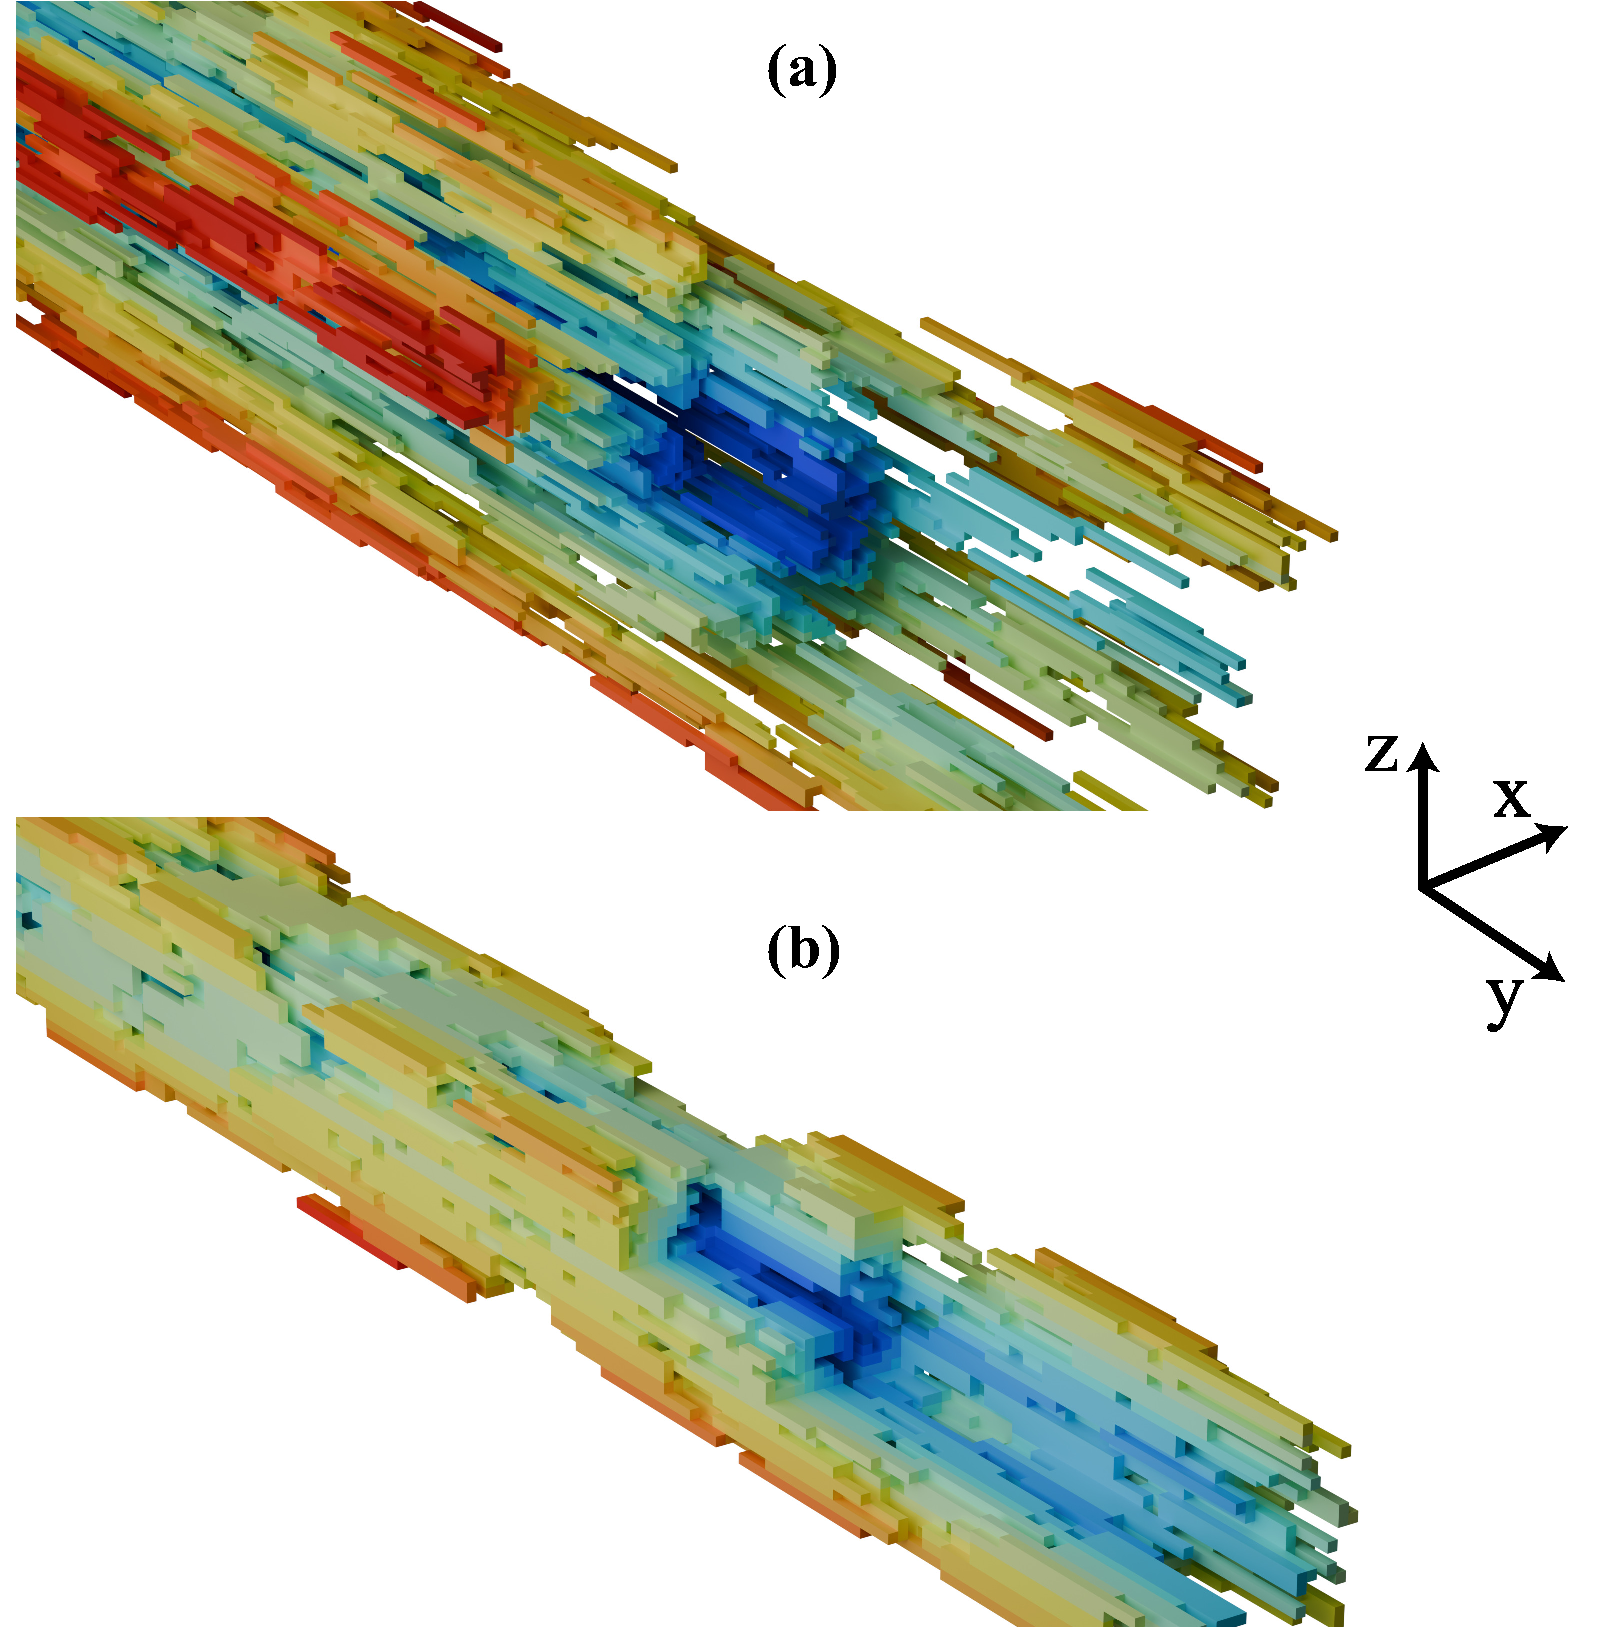
\includegraphics[width=0.7\textwidth]{figure_1.pdf}
	\caption{Representative fibril segments generated with the DLA algorithm containing 30,000 molecules. Panels $(a)$ and $(b)$ show typical fibrils obtained with $T_s = 2$ (short-term diffusion) and $T_s = 8192$ (long-term diffusion), respectively. Colors indicate the relative time of attachment, from early (blue) to late (red).}
	\label{fig_1}
\end{figure}

The generated fibrils exhibit complex, heterogeneous packing with internal voids whose prevalence depends strongly on $T_s$ (Fig.~\ref{fig_1}). For $T_s = 2$, the fibril displays an open architecture with visible gaps between molecular clusters. In contrast, for $T_s = 8192$, the structure becomes more compact and homogeneous, with substantially reduced void space.

Although fibril growth proceeds primarily along the longitudinal axis ($y$-direction), the influence of the surface diffusion parameter $T_s$ is most pronounced in the radial organization of the structure ($x$-$z$ plane), as illustrated in Fig.~\ref{fig_2}. At low $T_s$ (Fig.~\ref{fig_2}a), the projected cross-sections are open and branched. As $T_s$ increases, however, the packing becomes progressively more compact and regular, reaching a highly uniform configuration at $T_s = 8192$ (Fig.~\ref{fig_2}d). Since a higher local packing density implies a greater number of intermolecular contacts, this morphological transition suggests that fibrils formed at larger $T_s$ exhibit enhanced connectivity and mechanical stability \cite{Mohammadkhah2023}.

\begin{figure}[!htb]
	\centering
	\includegraphics[width=1.\textwidth]{figure_2.pdf}
	\caption{Representative examples of projected central segments ($x$-$z$ plane) for different values of $T_s$: (a) $T_s = 2$, (b) $T_s = 64$, (c) $T_s = 512$, and (d) $T_s = 8192$. The progression illustrates a clear transition from sparse, irregular morphology at low $T_s$ to dense, radially symmetric packing at high $T_s$. The color gradient (blue to red) represents the temporal sequence of molecular incorporation, from early-attached to recently added molecules.}
	\label{fig_2}
\end{figure}

To quantify how $T_s$ modulates fibril structure, we estimated the fractal dimension of the central segment, defined as the region extending from $y=-100$ to $y=100$. For each $T_s$, we generated 50 fibrils and isolated this central region from each. Within each central segment, we extracted 11 cross-sections at intervals of $18~\text{l.u.}$ between $y=-90$ and $y=90$, yielding a total of 550 cross-sections per $T_s$ value. For each cross-section, we computed the center of mass and the maximum radius enclosing all particles (segments of molecules); $R_{\text{max}}$ was subsequently defined as the largest of these 550 radii. The mass $m(R)$ was measured as the number of particles within a circular region of radius $R$ centered at the cross-section's center of mass. For each value of $R$ spanning from $R_{\text{min}} = 5~\text{l.u.}$ to $R_{\text{max}}$, we computed the mean mass $\langle m(R) \rangle$ by averaging over all 550 cross-sections \cite{Vicsek1991}. The fractal dimension $D_f$ was then estimated from the mass--radius scaling relation \cite{Giordano2012}:

\begin{equation}
	\langle m(R) \rangle \sim R^{D_{f}},
	\label{eq1}
\end{equation}
by performing a linear fit on a log-log plot of $\langle m(R) \rangle$ versus $R$.

As shown in Fig.~\ref{fig_3}, $D_f$ depends strongly on $T_s$, providing a quantitative measure of the morphological transition observed in Fig.~\ref{fig_2}. For $T_s = 2$, we find that $D_f = 1.708 \pm 0.005$, close to the characteristic value of two-dimensional diffusion-limited aggregation ($D_f \approx 1.71$) \cite{Witten1983}. As $T_s$ increases, $D_f$ rises and saturates at $D_f = 1.963 \pm 0.001$ for $T_s = 8192$, approaching the Euclidean limit of $D_f = 2.0$ expected for a compact two-dimensional disk. Thus, increasing post-attachment mobility drives a crossover from diffusion-limited, fractal packing to nearly space-filling cross-sections.

\rev{Here $D_f$ serves as an effective morphological descriptor of cross-sectional compaction, while the mechanics developed below is governed by two quantities measured directly on the three-dimensional backbone: the load-bearing area of each cross-section, $N(i)$, and the molecular coordination, $K$. Given the fibril radii accessible in simulation, $15$ to $40$ lattice units, the mass--radius scaling spans less than a decade, so the fitted slope tracks the structural transition toward compactness rather than an asymptotic scaling regime, and its value depends on the fitting window.}

\begin{figure}[h!]
	\centering
	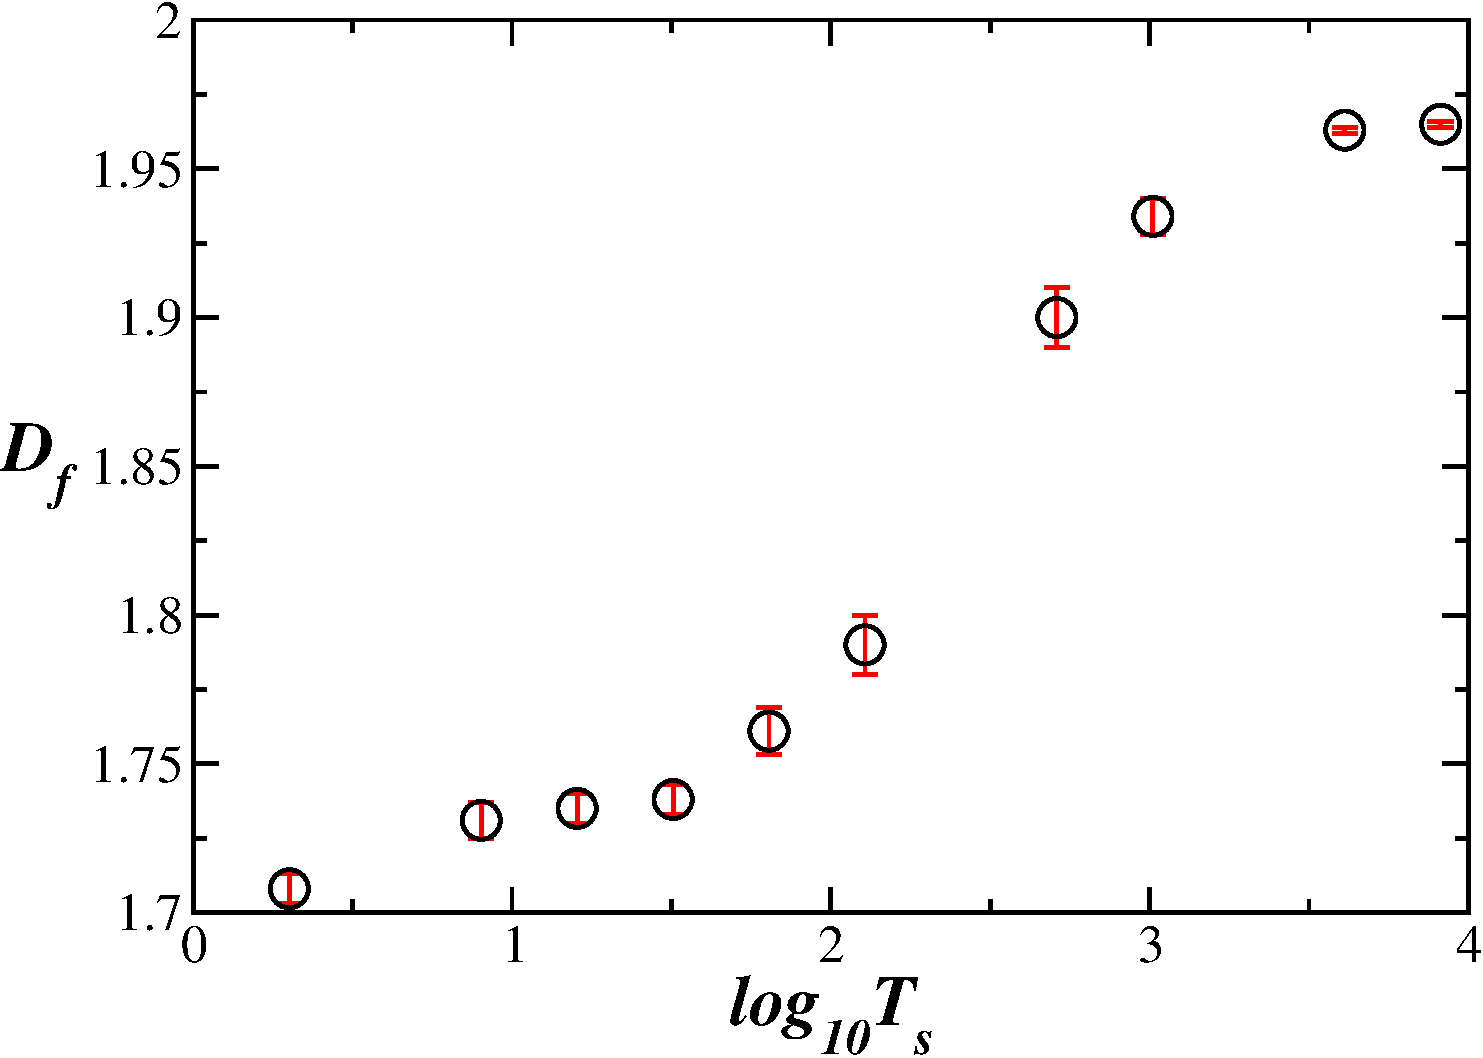
\includegraphics[width=0.7\textwidth]{figure_3.pdf}
	\caption{Average fractal dimension $D_f$ as a function of the diffusion parameter $T_s$ on a log-linear plot. Error bars are shown in red. The fractal dimension increases from $D_f = 1.708 \pm 0.005$ at $T_s = 2$ to $D_f = 1.963 \pm 0.001$ for $T_s = 8192$.}
	\label{fig_3}
\end{figure}		


\subsection{Mechanical Model for Fibril Rupture}

To connect the $T_s$-dependent fibril architecture to mechanical failure, we modeled rupture using a progressive, probabilistic fracture framework commonly employed for disordered networks \cite{z2019,Gilabert1987,Noguchi2024}. Because collagen molecules are represented as rigid rods that do not undergo continuous deformation prior to failure, we do not attempt to resolve deterministic crack propagation. Instead, intermolecular bonds fail stochastically under an applied axial force, and whole molecules detach from the load-bearing network with a stress-dependent probability. The procedure consists of:
$(i)$ isolating a trunk (force-carrying core) with dimensions $S_x = 17$, $S_y = 201$, and $S_z = 17$ l.u. \cite{Parkinson1997}. Truncation inevitably creates disconnected dangling ends that do not contribute to force transmission \cite{Herrmann1984}; we therefore
$(ii)$ identify the backbone (active skeleton) within the trunk prior to applying tensile loading \cite{Moreira2012}.

Backbone extraction proceeds in two passes. In the first pass, molecules at $y = 1$ are marked as active, and we scan upward to $y = S_y$, progressively marking molecules in contact with active ones; unmarked molecules are then removed. In the second pass, molecules at $y = S_y$ are marked as active, and we scan downward to $y = 1$ using the same connectivity rule; only molecules marked active after this pass are retained, defining the final backbone \cite{Parkinson1997} (Fig.~\ref{fig_4}).

\begin{figure}[h!]
	\centering
	
\includegraphics[width=\textwidth]{figure_4.pdf}
	\caption{(a) Two-dimensional visualization of an isolated fibril trunk used to extract the backbone. The circle highlights the region where the identification procedure starts ($y = 1$). (b) Example of the backbone identification procedure from left to right: molecules marked as active are highlighted in gray as connectivity is propagated along the trunk, yielding the final backbone.}
	\label{fig_4}
\end{figure}

With the backbone identified, we simulate the effects of axial tension along the fibril's axis ($y$) by progressively increasing a dimensionless force parameter $F$, where $F$ regulates the removal of molecules in a probabilistic fashion. At each cross-section $i$, we define the effective load-bearing area as the number of backbone segments intersecting that plane, $N(i)$. Each discrete segment is assigned a unit area on the lattice \cite{Parkinson1995}; assuming uniform load sharing, the local tensile stress at cross-section $i$ is:

\begin{equation}
	\sigma(i) = \dfrac{F}{N(i)}.
	\label{eq2}
\end{equation}

We assume that local failure occurs by rupturing intermolecular bonds so that molecules detach from each other rather than break \cite{Parkinson1997}. For a molecule spanning $n$ cross-sections, the mean stress is computed as the average of the local cross-sectional stresses:

\begin{equation}
	\sigma_{M} = \dfrac{1}{n}\sum_{i=1}^{n} \sigma(i).
	\label{eq3}
\end{equation}

A molecule's resistance to detach is assumed to scale with the number of intermolecular contacts it forms within the backbone \cite{Vater1979}. For each molecule, we count first-neighbor contacts for every segment in each intersected cross-section and sum these contributions to obtain the total coordination number $K$. The corresponding failure threshold is \rev{$\sigma^{\mathrm{th}} = K\sigma_c X$, where $X$ is a quenched strength variable drawn once per molecule before loading (Eq.~\ref{eq4}) and} $\sigma_c$ is the critical stress for bond rupture; we set $\sigma_c = 1$, assuming identical molecules. To simplify the model, both the applied force parameter $F$ and the critical stress $\sigma_c$ are treated as dimensionless quantities in arbitrary units. Hence, $\sigma_c = 1$ represents the normalized threshold for intermolecular bond rupture, which allows us to focus on relative mechanical behavior rather than absolute physical values.

\rev{The strength of each molecule is fixed before loading rather than resampled during it. Molecule $i$ draws a variable $X_i \in [0,1]$ once, with cumulative distribution}

\begin{equation}
	\rev{P(X_i \le x) = x^{m}, \qquad \sigma^{\mathrm{th}}_{i} = K_i \sigma_c X_i,}
	\label{eq4}
\end{equation}
\rev{and fails when its mean stress $\sigma_{M,i}$ exceeds its threshold $\sigma^{\mathrm{th}}_{i}$. Under this rule the probability that a molecule of coordination $K$ has failed once its mean stress reaches $\sigma$ is $(\sigma/K\sigma_c)^{m}$, so Eq.~(\ref{eq4}) is the original removal probability of our model read as a distribution of strengths; the weakening of a molecule as it loses neighbors, through $K$, is preserved unchanged. Here $m$ is the Weibull modulus, a dimensionless shape parameter controlling the scatter of the strengths~\cite{Parkinson1997,Jones2012}: larger $m$ yields a narrower distribution of rupture strengths, smaller $m$ a broader one. No Weibull modulus has been reported for single collagen fibrils, so we sweep $m \in \{1,2,3,5,10\}$ and retain $m = 2$, the value used by Parkinson et al.~\cite{Parkinson1997}, as the illustrative case in the figures.} Fig.~\ref{fig_5} schematically illustrates the calculation of $\sigma(i)$, $\sigma_{M}$, and $K$ for a representative molecule.

\rev{Equations~(\ref{eq2})--(\ref{eq4}) combine uniform load sharing within each cross-section with local, coordination-dependent molecular resistance. When a molecule is removed, $N(i)$ decreases only in the cross-sections it previously occupied, and the corresponding stress increase is shared uniformly among the remaining segments within each affected cross-section. The removal also reduces $K$ for the molecule's nearest neighbors, lowering their failure thresholds. Together these define a hybrid load-transfer mechanism: stress equilibrates uniformly among the active segments of each cross-section, while the failure thresholds respond to local coordination. Two features of the construction set it apart from the idealized limits. Stress is redistributed without any distance-dependent elastic kernel, so the coordination channel carries the only local information; and $N(i)$ varies along the fibril while molecules span different sets of cross-sections, so no single globally shared stress governs the bundle. The model therefore combines features of equal and local load sharing without mapping onto either limit.}

\begin{figure}[ht!]
	\centering
	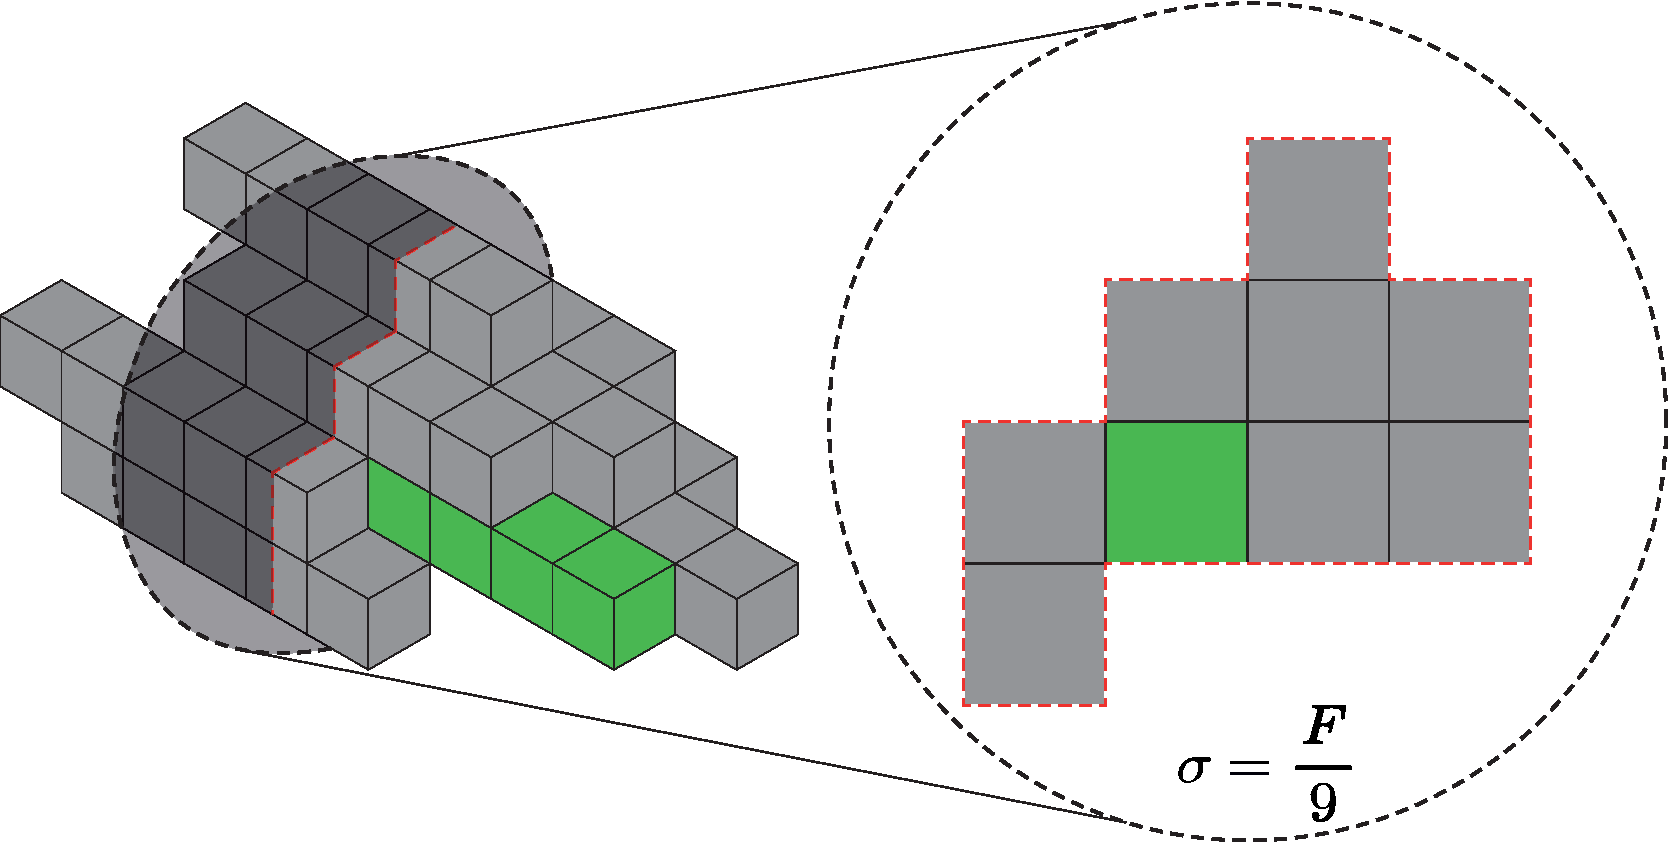
\includegraphics[width=0.9\textwidth]{figure_5.pdf}
	\caption{Schematic illustration of the computation of the removal probability $P_{R}$ for a representative molecule (green). Left: a portion of the backbone where each rectangle represents a molecule (drawn with five segments for clarity). The green molecule intersects multiple cross-sections; for each intersected cross-section $i$, the local stress is $\sigma(i)=F/N(i)$ (right; example with $N(i)=9$, giving $\sigma(i)=F/9$).}
	\label{fig_5}
\end{figure}

\rev{Because $\sigma_{M,i} = F a_i$ with $a_i = \langle 1/N(i) \rangle$ averaged over the cross-sections that molecule $i$ spans, every molecule has a well-defined failure force $F^{*}_{i} = K_i \sigma_c X_i / a_i$. Loading is quasi-static and extremal: the external force is raised continuously to the smallest $F^{*}_{i}$ present in the current configuration. At that fixed force the corresponding molecule fails; stresses and coordinations are then recomputed, molecules that have lost their connection to both ends of the specimen are removed, and the update is repeated until no molecule is above its threshold. The cascade terminates deterministically, and the configuration reached before each subsequent increase of the force is stable by construction, since every surviving molecule satisfies $F^{*}_{i} > F$. There is no force increment, no repeated sweep at fixed force, and no stopping criterion, and the model contains no physical time: it describes neither creep nor delayed rupture. Rupture is defined as the appearance of a completely void cross-section, signaling failure of the backbone. The steps of this process are schematized in Fig.~\ref{fig_6}.}

\begin{figure}[ht!]
	\centering
	\includegraphics[width=0.9\textwidth]{figure_6.pdf}
	\caption{Schematic view of the load-bearing backbone and the stages of the rupture process. (a) Two-dimensional view of the backbone subjected to an axial force $F$ along the $y$-axis. \rev{Each molecule (gray) carries a failure threshold $\sigma^{\mathrm{th}} = K\sigma_c X$ drawn once before loading (Eq.~\ref{eq4}); the external force is raised to the smallest failure force in the configuration, and the molecule that reaches it fails.} (b) Progressive damage after some molecules have been removed, represented by red dashed lines. (c) Rupture occurs when a cross-section becomes completely empty (solid lines), eliminating the continuous load path.}
	\label{fig_6}
\end{figure}

\rev{Because the molecular strengths are drawn at random, we sampled both the architecture and the disorder: for each value of $T_s$ and each value of $m$ we analyzed an ensemble of $200$ distinct fibrils, each containing $3\times 10^4$ molecules, and performed $50$ independent rupture realizations per fibril, that is, $10^4$ realizations for each of the fifty $(T_s, m)$ conditions. Realizations of the same fibril differ only in the drawn strengths. In each realization we recorded the molecules removed in every cascade and the external force at which the cascade occurred.}

\rev{To quantify the mechanical resistance of the fibrils we recorded, in each realization, the external force at which the backbone fails, $F_{\mathrm{rup}}$, and the fraction $\varphi$ of backbone molecules removed before the final cascade \cite{Parkinson1997}. Compact fibrils are markedly stronger. For $m = 2$ the mean rupture force grows from $151 \pm 36$ at $T_s = 2$ to $1532 \pm 218$ at $T_s = 8192$, an order of magnitude, with $83\%$ of the increase already attained at $T_s = 128$; per backbone molecule the force capacity grows by a factor of $2.6$, which follows from the higher coordination $K$ of compact packing (Fig.~\ref{fig_7}a). The rupture force varies between realizations of the same condition, with a coefficient of variation between $0.12$ and $0.29$.}

\rev{Damage before failure is modest, and it is not the gradual accumulation that the monotonic ensemble-averaged curve suggests. Depending on $T_s$ and $m$, only $9\%$ to $34\%$ of the backbone molecules are removed before the last cascade, and that cascade then removes $66\%$ to $91\%$ of what remains, in a single event at a single force. Rupture is therefore the sudden collapse of a still largely intact backbone rather than the endpoint of an accelerating loss of material; averaging over realizations that fail at different forces smooths the collapse into an apparent rapid rise. When the preterminal damage is plotted against the normalized force $F/F_{\mathrm{rup}}$, the curves collapse onto a common profile for $T_s \geq 32$ (Fig.~\ref{fig_7}b), so the dependence on architecture is carried almost entirely by $F_{\mathrm{rup}}$ itself.}

\begin{figure}[ht!]
	\centering
	
\includegraphics[width=\textwidth]{figure_7.pdf}
	\caption{\rev{(a) Mean rupture force $F_{\mathrm{rup}}$ as a function of $T_s$, for the five values of the Weibull modulus $m$; error bars are standard deviations over the $10^4$ realizations of each condition. (b) Fraction $\varphi$ of backbone molecules removed before the final cascade, as a function of the normalized force $F/F_{\mathrm{rup}}$, for $T_s = 2, 32, 128$ and $8192$ at $m = 2$; the curves collapse for $T_s \geq 32$.}}
	\label{fig_7}
\end{figure}

\rev{During rupture, molecules fail in cascades at constant external force. We define the avalanche as the complete cascade released by one increase of the force: the molecules whose thresholds are exceeded, together with those that lose their continuous load path as a consequence, all removed before the force is raised again. This is the set of molecules that fail between two consecutive increases of the external force, and it is the standard avalanche of fiber-bundle models, a form of crackling dynamics in driven disordered systems \cite{Jaeger1992,Godano1993,Beggs2003,Baraba1996,Alencar2001,Suki1994}. It contains no free parameter: its extent is set by the model, not by a force increment or by a connectivity criterion. Because load sharing within a cross-section is uniform (Eq.~\ref{eq2}), removals that are spatially disconnected within one cascade are nonetheless causally linked, each triggered by the same force increase or by the redistribution that followed it, so we do not partition cascades into connected clusters. The final cascade of each realization, which eliminates the last continuous load path and removes most of the remaining backbone, is a single terminal event and is excluded from the preterminal statistics analyzed below.}


% \rev{Figura do submetido com $\Psi$ retirada: o aglomerado conexo deixou de ser a definicao de avalanche.}

\rev{We analyze this collective behavior from the viewpoint of avalanche statistics in driven disordered fracture~\cite{Zapperi1997a,Zapperi1999,Zapperi1997b}. The avalanche size $s$ is the number of molecules removed in one cascade, as defined above, and we compute the distribution of preterminal cascade sizes for each of the fifty $(T_s, m)$ conditions, $6.1 \times 10^{7}$ events in total.}

\rev{The distributions are heavy at small sizes and cut off at large ones. Single-molecule cascades dominate the preterminal dynamics: they account for between $0.55$ and $0.78$ of all events depending on the condition, and are the majority in every one of the fifty, while the $99$th percentile of the cascade size lies between $8$ and $43$ molecules. No condition sustains a power law over more than one decade above the smallest size at which one could be fitted, so we tested the hypothesis rather than assuming it. On the raw, integer-valued cascade sizes of every condition we followed Clauset et al.~\cite{Clauset2009}: the lower cutoff was selected by minimizing the discrete Kolmogorov--Smirnov distance, the exponent estimated by exact discrete maximum likelihood, the pure power law tested by a semiparametric goodness-of-fit against synthetic replicas, and the fit compared with alternative distributions by normalized likelihood ratios. The pure power law is rejected in $48$ of the $50$ conditions, and the lognormal and the stretched exponential win the likelihood comparison in $49$: the cascade distributions are bounded by an intrinsic upper cutoff.}

\rev{The cutoff is a property of the model, not of the sampling. Above $T_s \approx 16$ it is insensitive to the architecture: at $m = 2$ the survival functions for $T_s = 16$, $128$, $1024$ and $8192$ nearly coincide, with $P(S>5)$ between $0.037$ and $0.042$ and the $99$th percentile of the cascade size at $12$ or $13$ molecules, while the most open architecture, $T_s = 2$, stands apart with $P(S>5) = 0.077$ and a $99$th percentile of $35$ (Fig.~\ref{fig_8}a). The width of the strength distribution does shift the balance between small and large events, in the direction expected: at $T_s = 128$, narrowing the disorder from $m = 1$ to $m = 10$ lowers the fraction of single-molecule cascades from $0.78$ to $0.59$ and raises the $99$th percentile from $8$ to $19$, because thresholds that lie closer together fail together (Fig.~\ref{fig_8}b). What does not change is the presence of the cutoff itself, which stays at a few tens of molecules over the whole grid. And each realization ends in one terminal cascade that removes most of the remaining backbone, so the process never settles into a stationary state with a diverging event scale: there is no healing mechanism by which a failed molecule could carry load again.}

% \rev{Paragrafo do submetido sobre crossover LLS -> GLS e mudanca de classe de universalidade: retirado.}

\begin{figure}[ht!]
	\centering
% Dados desta figura: Reviews/N10_cascade_survival/xmgrace/.
	
\includegraphics[width=\textwidth]{figure_8.pdf}
	\caption{\rev{Survival function $P(S > s)$ of the preterminal cascade sizes, on logarithmic axes. (a) For $T_s = 2, 16, 128, 1024$ and $8192$ at $m = 2$: the curves for $T_s \geq 16$ nearly coincide, and only the most open architecture stands apart. (b) For the five values of the Weibull modulus $m$ at $T_s = 128$. The terminal cascade of each realization is excluded. No power law is fitted, because in every condition fewer than one decade of cascade sizes lies above the smallest size at which a fit could begin.}}
	\label{fig_8}
\end{figure}

A direct consequence of avalanche-like rupture is that sudden stress drops should exist in the stress--strain curve, since avalanches propagate faster than the imposed loading rate \cite{Noguchi2024}. Although our model does not predict strain and thus cannot generate stress--strain curves, experimental evidence strongly supports this prediction. Gutsmann et al. \cite{Gutsmann2004} used force spectroscopy on single microfibrils and directly observed force drops caused by intermolecular cross-link ruptures. Svensson et al. \cite{Svensson2013} found clear stress drops in tensile tests of individual collagen fibrils, while Deng et al. \cite{Deng2024} observed similar drops in the stress--strain curves.

Our coarse-grained framework represents collagen molecules as rigid rods with restricted movement and no rotational diffusion. \rev{The rods have an aspect ratio of $18{:}1$, following Parkinson et al.~\cite{Parkinson1997}, substantially smaller than the $\approx 200{:}1$ ratio of real collagen monomers \cite{Buehler2008b}. While a fixed aspect ratio ensures a consistent geometry across all $T_s$, this simplification and the absence of rotational diffusion may quantitatively affect the coordination $K$, the load-bearing area $N(i)$, and the fractal dimension $D_f$. Our findings therefore capture the qualitative structural and mechanical trends of the model rather than exact quantitative predictions for biological fibrils.}

Intermolecular interactions are simplified via $T_s$, which lacks a direct mapping to interaction changes induced by biochemical conditions such as pH \cite{Jiang2004}. \rev{Calibrating $T_s$ against a specific experimental variable would require independent estimates of the incorporation and relaxation timescales, and remains beyond our scope \cite{Yang2009,Kalbitzer2018}.} Furthermore, while DLA captures the stochastic character of molecular accretion, biological fibrillogenesis is an actively regulated, energy-dependent process: collagen molecules first self-assemble into microfibrils---typically containing five molecules---which are then actively positioned and concatenated by the cell to form the growing fibril \cite{Kadler1996}\rev{, with fibronectin, integrins, and minor collagens organizing the process \cite{Canty2005,Kadler2008}. This is a further reason to read $T_s$ as an effective control parameter rather than as a proxy for a single biochemical condition}. Fracture is implemented as a probabilistic model, omitting detailed force transmission and internal bond-breaking mechanics \cite{RuizFranco2022,Provenzano2006}. Consequently, the model does not produce stress--strain curves or elastic moduli \cite{Innocenti2022-lp}. \rev{Within these limits, the framework captures the preterminal cascade dynamics reported above and an empirical association between structural compactness and mechanical resilience. Within the model that resilience is driven by the local load-bearing area $N(i)$ and the molecular coordination $K$, so structural compaction strengthens the fibril without requiring a self-similar load-transfer mechanism; consistently, the cascade statistics respond to the width of the strength distribution at fixed geometry.}

\section{Conclusion}

In this work, we combined a three-dimensional diffusion-limited aggregation model of collagen fibrillogenesis with a progressive probabilistic rupture model to connect assembly kinetics, fibril architecture, and failure statistics. Increasing the post-attachment surface diffusion parameter $T_s$ drives a clear morphological crossover from porous, fractal packing to nearly compact cross-sections: the measured fractal dimension rises from $D_f=1.708\pm0.005$ at $T_s=2$ to $D_f=1.963\pm0.001$ at $T_s=8192$. \rev{Mechanically, more compact fibrils are markedly stronger: for $m = 2$ the mean rupture force grows by an order of magnitude between $T_s = 2$ and $T_s = 8192$, and the force carried per backbone molecule grows by a factor of $2.6$. Only $9\%$ to $34\%$ of the backbone is lost before failure, which then arrives as a single terminal cascade removing most of what remains. The preterminal cascade-size distributions are dominated by single-molecule events and are cut off at a few tens of molecules everywhere on the grid; above $T_s \approx 16$ they are nearly independent of the architecture, while narrowing the strength distribution shifts weight from the smallest events toward the cutoff without removing it. The preterminal statistics and the rupture event therefore describe two distinct regimes: bounded damage, dominated by single-molecule events, while the backbone holds; and one unbounded event when it gives way.}

\rev{From a physical perspective, the growth of the rupture force with $T_s$ follows from the growth of the load-bearing area and of the molecular coordination, both of which lower the stress carried by each molecule at a given external force, and from the higher thresholds that a larger $K$ confers. The cross-sectional geometry and the failure statistics thus vary together over part of the range of $T_s$, and we report that as an empirical association within the model. Turning that empirical connection into a predictive theory is the natural next step, and it would require formulating the stress redistribution through a continuous disordered elastic medium carrying the cross-sectional porosity and the loss of lateral contacts, which the present discrete framework leaves open.} 

% \rev{Paragrafo do submetido comparando os expoentes medidos com 5/2 (ELS) e LLS: retirado.}

From a biological standpoint, the model developed here provides a simple mechanism to tune mechanical resilience of collagen fibrils, fibers and tissues by controlling assembly conditions that regulate compactness. \rev{Within the present model, a greater opportunity for post-attachment relaxation produces more compact fibrils with greater resistance to failure. Quantitative connections to physicochemical assembly conditions will require experimental estimates of molecular incorporation and rearrangement timescales, followed by calibration against measured fibril growth and morphology.} Future work should incorporate more realistic mechanics and time dependence---including elastic or viscoelastic deformation and evolving stiffness (e.g., due to cross-link dynamics or degradation)---to predict stress--strain behavior and track how the fiber modulus changes over time under load.

\section{Author Contributions}
All authors contributed equally to this work.

\section{Acknowledgments}
We thank the Brazilian agencies CNPq, CAPES, and FUNCAP for financial support.


% If in two-column mode, this environment will change to single-column
% format so that long equations can be displayed. Use
% sparingly.
%\begin{widetext}
% put long equation here
%\end{widetext}

% figures should be put into the text as floats.
% Use the graphics or graphicx packages (distributed with LaTeX2e)
% and the \includegraphics macro defined in those packages.
% See the LaTeX Graphics Companion by Michel Goosens, Sebastian Rahtz,
% and Frank Mittelbach for instance.
%
% Here is an example of the general form of a figure:
% Fill in the caption in the braces of the \caption{} command. Put the label
% that you will use with \ref{} command in the braces of the \label{} command.
% Use the figure* environment if the figure should span across the
% entire page. There is no need to do explicit centering.

% \begin{figure}
% \includegraphics{}%
% \caption{\label{}}
% \end{figure}

% Surround figure environment with turnpage environment for landscape
% figure
% \begin{turnpage}
% \begin{figure}
% \includegraphics{}%
% \caption{\label{}}
% \end{figure}
% \end{turnpage}

% tables should appear as floats within the text
%
% Here is an example of the general form of a table:
% Fill in the caption in the braces of the \caption{} command. Put the label
% that you will use with \ref{} command in the braces of the \label{} command.
% Insert the column specifiers (l, r, c, d, etc.) in the empty braces of the
% \begin{tabular}{} command.
% The ruledtabular enviroment adds doubled rules to table and sets a
% reasonable default table settings.
% Use the table* environment to get a full-width table in two-column
% Add \usepackage{longtable} and the longtable (or longtable*}
% environment for nicely formatted long tables. Or use the the [H]
% placement option to break a long table (with less control than 
% in longtable).
% \begin{table}%[H] add [H] placement to break table across pages
% \caption{\label{}}
% \begin{ruledtabular}
% \begin{tabular}{}
% Lines of table here ending with \\
% \end{tabular}
% \end{ruledtabular}
% \end{table}

% Surround table environment with turnpage environment for landscape
% table
% \begin{turnpage}
% \begin{table}
% \caption{\label{}}
% \begin{ruledtabular}
% \begin{tabular}{}
% \end{tabular}
% \end{ruledtabular}
% \end{table}
% \end{turnpage}

% Specify following sections are appendices. Use \appendix* if there
% only one appendix.
%\appendix
%\section{}

% If you have acknowledgments, this puts in the proper section head.
%\begin{acknowledgments}
% put your acknowledgments here.
%\end{acknowledgments}

% Create the reference section using BibTeX:
\bibliography{apssamp}

\end{document}
%
% ****** End of file apstemplate.tex ******
